\documentclass[review]{elsarticle}
\usepackage{lineno,hyperref,amssymb,graphicx,booktabs}

\modulolinenumbers[5]
\journal{Nuclear Instruments and Methods in Physics Research A}


% Note from Jeff: Our previous NMOR article was 20 pages in this
% format, which became about 6 pages in the final paper in NIMA.


%%%%%%%%%%%%%%%%%%%%%%%
%% Elsevier bibliography styles
%%%%%%%%%%%%%%%%%%%%%%%
%% To change the style, put a % in front of the second line of the current style and
%% remove the % from the second line of the style you would like to use.
%%%%%%%%%%%%%%%%%%%%%%%

%% Numbered
%\bibliographystyle{model1-num-names}

%% Numbered without titles
%\bibliographystyle{model1a-num-names}

%% Harvard
%\bibliographystyle{model2-names.bst}\biboptions{authoryear}

%% Vancouver numbered
%\usepackage{numcompress}\bibliographystyle{model3-num-names}

%% Vancouver name/year
%\usepackage{numcompress}\bibliographystyle{model4-names}\biboptions{authoryear}

%% APA style
%\bibliographystyle{model5-names}\biboptions{authoryear}

%% AMA style
%\usepackage{numcompress}\bibliographystyle{model6-num-names}

%% `Elsevier LaTeX' style
%\bibliographystyle{elsarticle-num}
%%%%%%%%%%%%%%%%%%%%%%%

\begin{document}

\begin{frontmatter}

\title{Sensitivity of Fields within Magnetically Shielded Volumes to
  Changes in Permeability}

\author[manitoba]{T. Andalib\corref{mycorrespondingauthor}}
\cortext[mycorrespondingauthor]{Corresponding author}
\ead{andalibt@myumanitoba.ca}
\author[winnipeg,manitoba]{C.P. Bidinosti}
\author[winnipeg,manitoba]{R.R. Mammei}
\author[winnipeg,manitoba]{J.W. Martin}
\author[winnipeg]{D. Ostapchuk}

\address[winnipeg]{Physics Department, The University of Winnipeg, 515 Portage Avenue, Winnipeg, MB, R3B 2E9, Canada}
\address[manitoba]{Department of Physics and Astronomy, University of Manitoba, Winnipeg, MB R3T 2N2, Canada}


\begin{abstract}
Future experiments seeking to measure the neutron electric dipole
moment (nEDM) require stable and homogeneous magnetic fields.  The
stability of the magnetic field within a magnetically shielded volume
is influenced by a number of factors.  In this paper, we study one of
these factors, which is the dependence of the internally generated
field on the permeability of the material.  We also provide
measurements of the temperature-dependence of the permeability of the
material, and indicate the extrapolation yet required to adequately
use these measurements to design future nEDM experiments.
\end{abstract}

\begin{keyword}
Magnetic Shielding \sep Neutron Electric Dipole Moment \sep Magnetic Field Stability
\end{keyword}

\end{frontmatter}

\linenumbers

\section{Introduction}

The next generation of neutron electric dipole moment (EDM)
experiments aim to measure the EDM $d_n$ with proposed precision
$\delta d_n\lesssim
10^{-27}$~e-cm~\cite{bib:nedm1,bib:nedm2,bib:nedm2.5,bib:nedm3,bib:nedm3.5,bib:nedm4,bib:nedm5,bib:nedm6,bib:nedm6.5}.
In the previous best experiment \cite{bib:pendlebury}, which discovered
$d_n<3\times 10^{-26}$~e-cm (90\% C.L), effects related to magnetic field
homogeneity and instability were found to dominate the systematic
error.  A detailed understanding of passive and active magnetic
shielding, magnetic field generation within shielded volumes, and
precision magnetometry is expected to be crucial to achieve the
systematic error goals for the next generation of experiments.  Much
of the R\&D effort for these experiments is focused on careful design
and testing of various magnetic shield geometries with precision
magnetometers~\cite{bib:brys,bib:afach,bib:fierlingerroom,bib:sturmthesis,bib:patton}.

%%%%%%%%%%%%%%%%%%%%%%%%%%%%%%%%%%%%%%%%%%%%%%%%%%%%%%%%%%%%%%%%%%%%55
% Taraneh
%%%%%%%%%%%%%%%%%%%%%%%%%%%%%%%%%%%%%%%%%%%%%%%%%%%%%%%%%%%%%%%%%%%%55
%\begin{itemize}
%\item General requirements on field, stability of field, stability of gradient.
%\item List all possible factors that can affect field stability -
 % degaussing, vibrations, etc. possibly with additional references.
%\item State the problem addressed in this paper (changes in $\mu$) and
 % the result.
%\end{itemize}
The nEDM experiment at TRIUMF aims to determine $\delta d_n \sim 10^{-27}$ e$\cdot$cm. This level of precision requires a 1 $\mu$T magnetic field with the homogeneity of $<$ 1 nT/m and the stability of pT over the UCN free-precession time.\\
Any slight mechanical and temperature changes of the experiment setup as well as the demagnetization of passive shielding will affect the stability of the magnetic field within the measurement volume.\\
The passive shields for the nEDM experiments are made of highly permeable materials such as Mu-Metal which is a Ni-Fe alloy that allows measurements at low frequency magnetic fields. Ni-Fe alloys operate at room temperature and are sensitive to small temperature variations which affects the electromagnetic behaviour of the material such as the magnetic permeability, $\mu$ \cite{bib:couderchon}. For these type of alloys $\mu$ depends also on the annealing process \cite{bib:gupta}. The temperature dependence of $\mu$ has been measured from two different approaches and the overall result found to be 0.1\%/K $<\frac{1}{\mu} \frac{d\mu}{dT}<$2.3\%/K.


\section{Sensitivity of Internally Generated Field to Permeability of the Shield $B_0(\mu)$}

\subsection{Analytical Calculations in Spherical (and Cylindrical) Geometry}

%%%%%%%%%%%%%%%%%%%%%%%%%%%%%%%%%%%%%%%%%%%%%%%%%%%%%%%%%%%%%%%%%%%%55
% Taraneh
%%%%%%%%%%%%%%%%%%%%%%%%%%%%%%%%%%%%%%%%%%%%%%%%%%%%%%%%%%%%%%%%%%%%55
%\begin{itemize}
%\item State basic physics of problem, define reaction factor, note
%  return flux through shield, etc.
%\item State formulae and results for reasonable parameters.
%\item Possibly one graph of $B_0(\mu)$ with both geometries.
%\end{itemize}

The presence of a coil inside the innermost passive shield turns the shield into a return yoke and its due to the penetration of the magnetic field flux into the magnetic shield. The ratio of the magnetic field inside the coil in the presence of the magnetic shield to the coil in free space can be called the reaction factor $C$ which is $>$ 1 for spherical and cylindrical geometries \cite{bib:bidinosti}. The coupling of the coil to the innermost layer of the magnetic shield suggests that any changes in the properties of the magnetic shield gives rise to a change in the internal field. One of these properties is $\mu$ which is of significant importance because of the high permeability of the passive shields. As a result, the stability of the magnetic shields contributes to the stability of the internal field.

From Refs. \cite{bib:smythe, bib:ferraro} for a zonal surface current
\begin{equation}
\bold{F}=- \sum_{n=1} ^{\infty} \frac{C_n}{l} P^1 _n (u) \hat{\phi}
\end{equation}
bound on a sphere with radius $l$ the magnetic field at $r < l$ and $r>l$ is calculated.
The case of an ideal spherical surface current ($n=1$) inside a spherical shell with inner radius $a$ and outer radius $b$ has been analytically calculated considering the following boundary conditions

\begin{equation}
\frac{1}{\mu_0} B_{\theta} (a^-) = \frac{1}{\mu} B_{\theta}(a^+)
\end{equation}
\begin{equation}
\frac{1}{\mu}B_{\theta}(b^-)=\frac{1}{\mu_0}B_{\theta}(b^+).
\end{equation}
Fig. \ref{fig:Magnetic_Field} shows the magnetic field $B$ as a function of relative $\mu$ for $l=0.53$ m, $a=0.57$ m and a thickness of 1.5 mm for the shield which are comparable to the dimensions of the ILL nEDM experiment setup \cite{bib:baker, bib:knecht}.
\begin{figure}[h!]
\begin{center}
   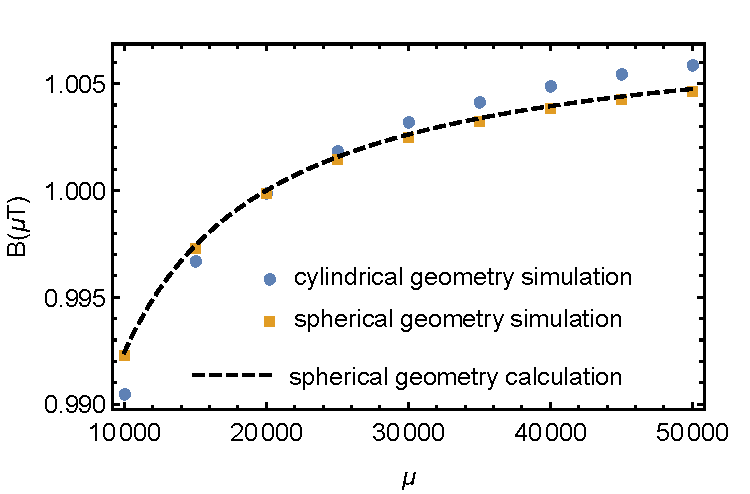
\includegraphics[width=0.6\textwidth]{femm_and_calcs.pdf}
    \caption{This graph shows magnetic field in $\mu$T as a function of relative magnetic permeability $\mu$ for an ideal spherical surface current of radius $0.53$ m inside a spherical shell of inner radius 0.57 m and a thickness of 1.5 mm. (fix the caption)}
    \label{fig:Magnetic_Field}
    \end{center}
\end{figure} 
For a 10\% change in relative $\mu$ from 20000 to 22000, the magnetic field changes by 0.7 nT.



\subsection{Magnetostatic Simulation Results}

%%%%%%%%%%%%%%%%%%%%%%%%%%%%%%%%%%%%%%%%%%%%%%%%%%%%%%%%%%%%%%%%%%%%55
% Jeff; need to decide graphs with Taraneh.
%%%%%%%%%%%%%%%%%%%%%%%%%%%%%%%%%%%%%%%%%%%%%%%%%%%%%%%%%%%%%%%%%%%%55
\begin{itemize}
\item I think it would be easy to provide results in axisymmetric
  geometries from FEMM.
\item If any result is available from OPERA, it could be included here.
\item Results should be for a restricted set of possible nEDM coils.
\item quote reaction factors?
\item One graph?  % probably the same graph as above
\end{itemize}

\subsection{Self-Shielded Coils}

%%%%%%%%%%%%%%%%%%%%%%%%%%%%%%%%%%%%%%%%%%%%%%%%%%%%%%%%%%%%%%%%%%%%55
% Chris B advises to make this section much more vague and shorter.
% (Jeff can do)
%%%%%%%%%%%%%%%%%%%%%%%%%%%%%%%%%%%%%%%%%%%%%%%%%%%%%%%%%%%%%%%%%%%%55
\begin{itemize}
\item Explain principle (reaction factor = 1, or no field at shield so
  no return flux)
\item Simple analytic results - reaction factor is identically unity.
\item FEMM/OPERA - demonstrate that sensitivity is reduced by factor
  of XX for simple geometry.
\item One graph, or include on previous graph?
\end{itemize}

\subsection{Summary of $B_0(\mu)$}
%%%%%%%%%%%%%%%%%%%%%%%%%%%%%%%%%%%%%%%%%%%%%%%%%%%%%%%%%%%%%%%%%%%%55
% Taraneh
%%%%%%%%%%%%%%%%%%%%%%%%%%%%%%%%%%%%%%%%%%%%%%%%%%%%%%%%%%%%%%%%%%%%55
%Insert summary here.
For the shield-coupled coils the magnetic field in the region interior to the coil is coupled to the properties of the shell which is caused by the penetration of the magnetic field into the shell material. However, for an ideal case such as a spherical coil inside a spherical shell the dependence of the magnetic field $B$ to $\mu$ is not very strong. This coupling can be much reduced by replacing the shield-coupled coils with the self-shielded coils.

\section{Measurements of $\mu(T)$}

\subsection{Previous Measurements and their Relationship to nEDM Experiments}
Couderchon et al. measured the thermal variation of $\mu$ of two different Ni-Fe alloys in a low field and they found $\frac{1}{\mu}\frac{d \mu}{dT}\simeq$ 1 $\%/K$ at room temperature \cite{bib:couderchon}. Based on the data sheet of a similar material, $\mu$ would depend on temperature as $\frac{1}{\mu} \frac{d \mu}{dT} \simeq $ 0.3-0.7 \%/K \cite{bib:kruppvdm}. These are measurements of the temperature dependence of $\mu$ at frequencies much higher than the nEDM experiment (50 Hz compared to 0.01Hz). In addition, the applied magnetic field $H$ and magnetic flux density $B$ in these experiments are not clear while the static magnetic field for the nEDM experiment is about 1 $\mu$T.

Here two different approaches to measure temperature dependence of $\mu$ were pursued. To elucidate the behavior of our passive Mu-metal shields, experiments were done using two witness cylinders, which are smaller open-ended cylinders (6" in length) made of the same material and annealed at the same time as our big prototype shields. We therefore expect they have the same magnetic properties as the big passive shields, but they are much smaller and easier to perform measurements with.
%\begin{itemize}
%\item Coucheron et al.?
%\item Krupp-VDM data sheet?
%\item Proper literature search on past measurements of $\mu(T)$.
%\item State caveats in order to use these:  dependence on B, H, f.
%\item State typical B, H, f that nEDM needs.  Motivates additional
 % measurements.
%\end{itemize}

\subsection{Axial Shielding Factor Measurements}
In the first approach, the witness cylinder was used as a magnetic shield. 
The general idea is to measure any changes in the shielding factor corresponding to a temperature change of the witness cylinder. 
A solenoid producing a known homogeneous magnetic field was placed outside the witness cylinder as shown in Fig. \ref{fig:geometry}.
A fluxgate magnetometer measured the magnetic field inside the witness cylinder while the temperature of the shield was measured.
The solenoid current was varied sinusoidally at typically 0.01 to 10 Hz.
The signal from the fluxgate was demodulated by a lock-in amplifier providing the in-phase and out-of-phase components of the signal.

\begin{figure}[h!]
\begin{center}
   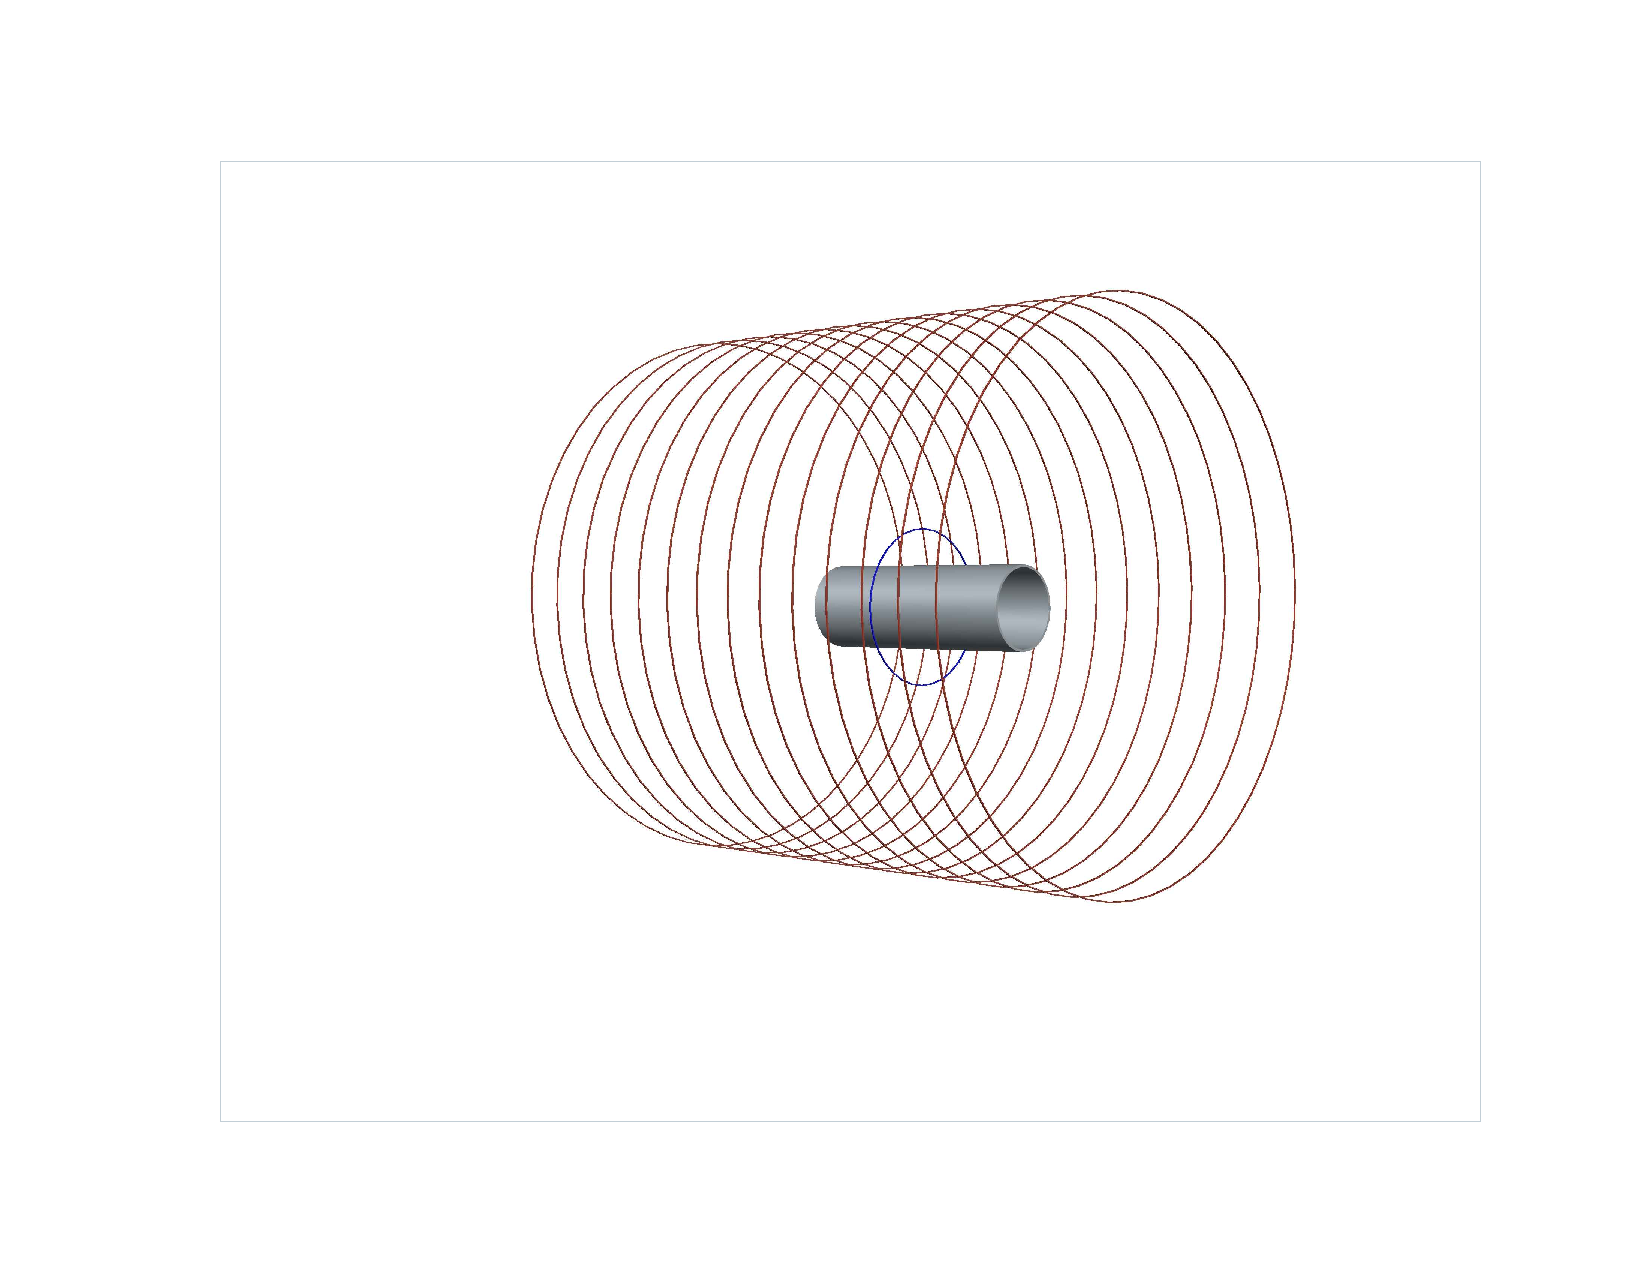
\includegraphics[width=0.8\textwidth]{geometry.pdf}
    \caption{This figure shows the setup of the axial shielding factor measurement. The witness cylinder is placed inside a solenoid. The axis of symmetry is along the z axis. The windings of the solenoid is shown in red. The blue coil with one turn is coupled to the witness cylinder.   }
    \label{fig:geometry}
    \end{center}
\end{figure} 

An example of the typical data acquired is shown in Fig. \ref{fig:B_vs_Temp}. Graph (a) shows the temperature of the witness cylinder over four days. The temperature changes are about 3.5$^\circ$C and are caused by temperature variations of the room. The magnetic field $B$ is the sum, in quadrature, of the in-phase and out-of-phase components. For $f\lesssim 1$ Hz most of the measured fluxgate signal is in the in-phase component. The magnetic field tracks the temperature trend in an opposite way which is shown in graph (b). The slope of the graph (c) has been calculated by using a linear fit to the data. In general, we measured 0.3 \%/K $< \vert \frac{1}{B} \frac{dB}{dT} \vert <$ 2.3 \%/K with the sign being negative. The range embodies the typical nonlinearities in the data (for example, those seen in graph (c) of Fig. \ref{fig:B_vs_Temp}.), and so we adopt this as an uncertainty. Through a comprehensive set of systematic studies, the source of the nonlinearities could not be found. We suspect it is due to a combination of mechanical stability and properties of the material that cannot be embodied by a simple temperature slope. Thus the experiment tends to set a scale and sign for the possible temperature dependence, rather than a value.
  \begin{figure}[h!]
\begin{center}
   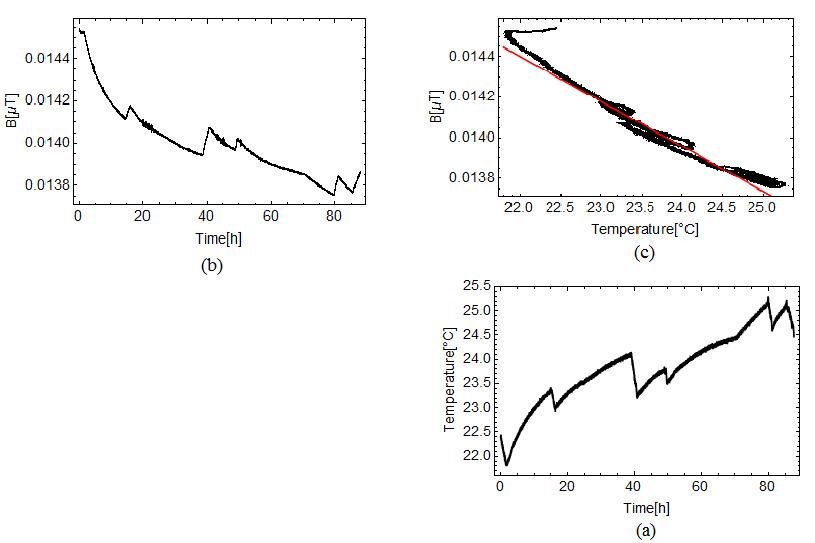
\includegraphics[width=0.5\textwidth]{B_vs_T.png}
    \caption{These graphs show data of temperature dependence of the magnetic field taken over 80 hours. Graph (a) shows the temperature of the witness cylinder in $^\circ$C as a function of time. Graph (b) shows the magnetic field inside the witness cylinder at the center in $\mu$T versus time and graph (c) shows the magnetic field in $\mu$T versus temperature in $^\circ$C. The red line is the linear fit to data. At 22$^\circ$C, $\vert \frac{1}{B}\vert \vert \frac{dB}{dT}\vert\simeq -1.5 \% /K.$ }
    \label{fig:B_vs_Temp}
     \vspace{-2.em}
    \end{center}
\end{figure} 

To relate this data to $\mu $(T), finite element simulations in FEMM and OPERA were done. From these simulations the ratio $\frac{\mu}{B} \frac{dB}{d\mu}$ was calculated in a model where $\bold{B} = \mu \bold{H}$ and $\mu $ is a constant i.e. the material is treated as being linear. The term $\frac{\mu}{B}\frac{dB}{d\mu}\neq 0$ because the witness cylinders are open ended. Combining the measurement and the simulations, the temperature dependence of effective $\mu$ (at $\mu$=20000) can be calculated by
\begin{equation}
\frac{1}{\mu}\frac{d\mu}{dT}= -\frac{\frac{1}{B}\frac{dB}{dT}}{\frac{\mu}{B}\frac{dB}{d\mu}}.
\end{equation}

The dominant systematic uncertainties in this experiment are due to mechanical stability and field profile.  In this model it was found that 0.6\%/K $\lesssim\frac{1}{\mu}\frac{d\mu}{dT}\lesssim 2.3\%$/K.
%\begin{itemize}
%\item Describe experimental setup and important considerations
%  (e.g. relationship of data to effective $\mu$)
%\item Explain B, H, f, and dominant systematic effects.
%\item One figure of experimental setup?
%\item One data graph?
%\item State overall result and systematic error.
%\end{itemize}

\subsection{Transformer Core Measurements}
In second approach, the witness cylinder was used as the core of a transformer. Two coils (primary and sense coils) were wound on the witness cylinder. The primary coil generated an AC magnetic field while the sense coil measured the sense voltage caused by the magnetic flux inside the witness cylinder. This experiment is done at 1 Hz and as small as possible $H$, to measure the slope of minor loops near the origin of the $B-H$ space. In lower frequencies, noise dominated the actual signal.
The temperature of the core was measured concurrently as the sense voltage.
The measured voltage induced on the sense coil, is proportional to $\mu$.
The measurements show a range of 0.1\%/K to 2\%/K for $\frac{1}{\mu}\frac{d\mu}{dT}$, again assuming the material to be linear.

In all transformer measurements, the sense voltage from the sense coil was demodulated by a lock-in amplifier. In Fig. \ref{fig:data_and_simulation} the in-phase component $Y$ and out-of-phase component $X$ of the sense signal as a function of applied $H$ field at 1 Hz are shown. In the ideal case where the material is linear, the $X$ component should be zero. The ratio of the $X/Y$ depends on both the applied frequency and the position on the $B-H$ region. We were interested in regions where $\vert Y \vert > \vert X \vert $ in which the material behaves as being linear and the $\vert H \vert $ values correspond to $\vert X \vert < \vert X_{max} \vert$ while still being able to get a good signal to noise ratio.


A concern in both measurements is that, the material is not linear. There are other effects such as hysteresis, saturation, eddy currents and skin depth which all contribute to the measured signal and so it is not possible to embody the results as a single parameter. 
To check the sensitivity of the sense coil demodulated voltage to these effects, a theoretical model of the hysteresis (Jiles-Atherton model) was used \cite{bib:jiles}, see Fig.  \ref{fig:data_and_simulation}. 

The key parameters of Jiles-Atherton model are saturation magnetization $M_s$, mean field parameter $\alpha$ which represents interdomain coupling, $a$ with the dimensions of magnetic field which characterizes the shape of anhysteretic magnetization, bulk magnetization $M$ and the magnetic field $H$. A shown in Fig. \ref{fig:data_and_simulation}, trends in the measurements and simulations are fairly consistent.

Some measurements regarding degaussing have been done to study how removing magnetization effects the sense voltage. Degaussing (idealizing) magnetic shields means to saturate the shields by applying a very large magnetic field and then slowly ramping this applied field down to zero. In most cases, degaussing helped to increase the signal and hence $\mu$.

\begin{figure}[h!]
\begin{center}
   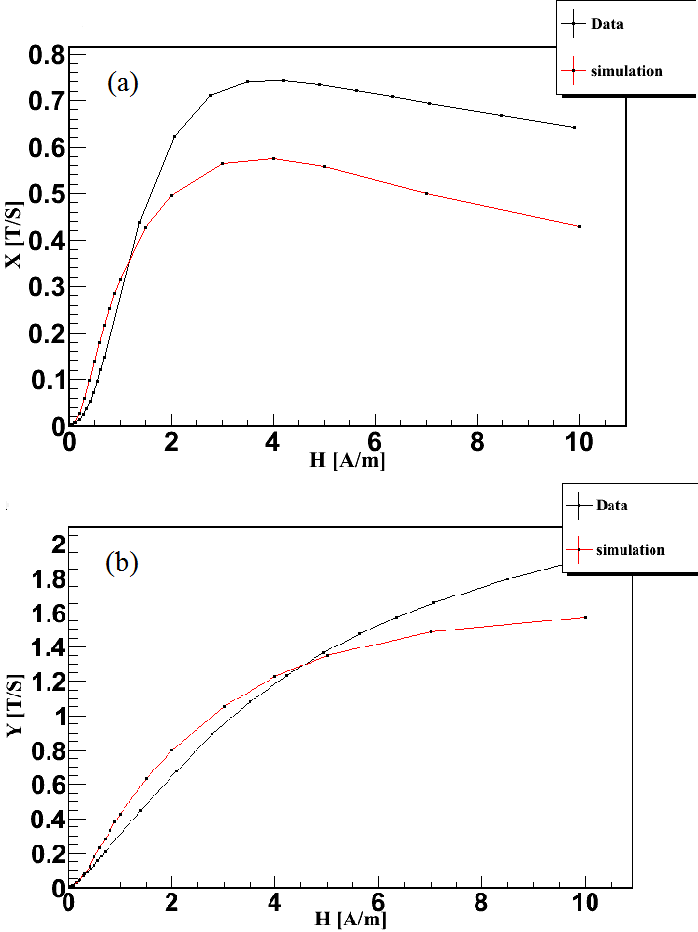
\includegraphics[width=0.5\textwidth]{data_and_simulation3.PNG}
    \caption{These graphs represent the sense voltage as a function of applied $H$ field at 1 Hz. Graph (a) shows the out-of-phase component $X$ of the measured sense voltage as well as the simulation. Graph (b) shows the in-phase component $Y$ of the signal and its simulation.}
    \label{fig:data_and_simulation}
    \end{center}
\end{figure} 

%\begin{itemize}
%\item Describe experimental setup and important consdierations (e.g. relationship of data to effective $%\mu$)
%\item Explain B, H, f, and dominant systematic effects.
%\item Understanding in terms of Jiles-Atherton.  Complications that
 % this does not translate well into ``$\mu$''.
%\item One data graph?  (Perhaps the Jiles-Atherton one?)
%\item State overall result and systematic error.
%\end{itemize}
%%%%%%%%%%%%%%%%%%%%%%%%%%%%%%%%%%%%%%%%%%%%%%%%%%%%%%%%%%%%%%%%%%%%%%
% Taraneh, can you write text up to this point?
%%%%%%%%%%%%%%%%%%%%%%%%%%%%%%%%%%%%%%%%%%%%%%%%%%%%%%%%%%%%%%%%%%%%%%

\subsection{Summary of $\mu(T)$}

%Insert Summary Here.
 The overall error bar in $\mu$ from both measurement techniques is 0.1\%/K $\leq \frac{1}{\mu}\frac{d\mu}{dT} \leq$ 2.3 \%/K and it is consistent with previous data.
Comparing to the static nEDM experiment with $f < 0.01$ Hz, these measurements are mostly done at frequencies close to 1 Hz. Hence, the effective $\mu$ extracted from these type of experiments give
only a qualitative information on the actual nEDM experiment situation and to reach higher accuracy the nEDM experiment has to be built. 
\section{Summary and Conclusions}

\begin{itemize}
\item We determined $dB_0/d\mu$.  For reasonable parameters its $\sim$ XXX.  For self-shielded it's reduced by a factor of XXX for realistic windings.
\item We measured $d\mu/dT$.  We constrained it to be in the range 0.1
  to 2.3 percent per Kelvin.  Dominant errors are XXX for each method.
  Neither method is for correct B, H, f.  Both methods are very
  difficult to achieve consistent sub-percent determinations, but tend
  to agree on sign and magnitude of problem.
\item Results imply temperature stability to XXX Kelvin for stability
  goal of XXX pT.  Show that this could be a dominant issue for
  stability for future experiments.  Not addressed by many other
  measurements which tend to focus on stability at zero field or
  overall stability in full EDM experiment.
\item Future work: build full EDM experiment.  Capability of various
  internal coil geometries and best achievable temperature stability
  are both important to success.
\end{itemize}

%\section{To Do List}

%\begin{enumerate}
%\item Collect graphs and figures.
%\begin{enumerate}
%\item Analytical comparison reaction factor vs. $\mu$ for
 % sphere and/or cylinder with reasonable geometry/$\mu$.
%\item Same or additional comparison for more realistic geometry in
%  simulation.  May include self-shielded geometry.
%\item Axial shielding factor figure of setup.
%\item Axial shielding factor data.
%\item Transformer core Jiles-Atherton comparison?
%\end{enumerate}
%\item Write.
%\end{enumerate}

\section*{References}

\bibliography{mybibfile}
\begin{thebibliography}{00}

\bibitem{bib:nedm1} S. N. Balashov {\it et al.}, arXiv:0709.2428.

\bibitem{bib:nedm2} A. P. Serebrov {\it et al.}, JETP Lett. {\bf 99}, 4
  (2014).

\bibitem{bib:nedm2.5} A. P. Serebrov {\it et al.}, Physics Procedia {\bf
  17}, 251 (2011).

\bibitem{bib:nedm3} K. Kirch, AIP Conf. Proc., Vol. 1560, pp. 90-94
  (2013).

\bibitem{bib:nedm3.5} C. A. Baker, {\it et al.}, Physics Procedia {\bf
  17}, 159 (2011).

\bibitem{bib:nedm4} Y. Masuda, K. Asahi, K. Hatanaka, S.-C. Jeong,
  S. Kawasaki, R. Matsumiya, K. Matsuta, M. Mihara, and Y. Watanabe,
  Phys. Lett. A {\bf 376}, 1347 (2012).

\bibitem{bib:nedm5} I. Altarev, {\it et al.}, Nuovo Cim. C {\bf
  35}, 122 (2012).

\bibitem{bib:nedm6} R. Golub and S. K. Lamoreaux, Phys. Rept.  {\bf
  237}, 1 (1994).

\bibitem{bib:nedm6.5} T. M. Ito (the nEDM collaboration),
  J. Phys. Conf. Ser. {\bf 69} 012037, 2007.

\bibitem{bib:baker} C. A. Baker, {\it et al.}, Phys. Rev. Lett. {\bf
  97}, 131801 (2006).

\bibitem{bib:brys} T. Bry\'s, {\it et al.}, Nucl. Instrum. Meth. A
  {\bf 554}, 527 (2005).

\bibitem{bib:afach} S. Afach, {\it et al.}, J. Appl. Phys. 116, 084510 (2014).

\bibitem{bib:fierlingerroom} I. Altarev, {\it et al.}
  Rev. Sci. Instrum. {\bf 85}, 075106 (2014).

\bibitem{bib:sturmthesis} M. Sturm, Masterarbeit, T.U. Muenchen (2013).

\bibitem{bib:patton} B. Patton, E. Zhivun, D. C. Hovde, and D. Budker,
  Phys. Rev. Lett. 113, 013001 (2014).
\bibitem{bib:couderchon} G. Couderchon, J. F. Tiers, J. Magn. Magn. Mat. 26(1):196-214 (1982).

\bibitem{bib:bidinosti} C. P. Bidinosti {\it et al.}, AIP Advances 4, 047135 (2014).

\bibitem{bib:smythe} W. R. Smythe, McGraw Hill (1950).

\bibitem{bib:ferraro} V. C. A. Ferraro, Athalone Press (1967).

\bibitem{bib:gupta} Kiran Gupta, K. K. Raina, S. K. Sinha, J. Alloys Compd, 429(1):357-364 (2007).

\bibitem{bib:knecht} A. Knecht, Dissertation, UZH Zurich (2009).

\bibitem{bib:kruppvdm} KruppVDM Magnifer 7904, MDS no. 9004 (2000).

\bibitem{bib:jiles} D. C. Jiles, D. L. Atherton,  J. Magn. Magn. Mat. 61(1-2):48-60, (1986).

\bibitem{bib:pendlebury} J. M. Pendlebury {\it et al.}, Phys. Rev. D 92, 092003 (2015).

\end{thebibliography}

\end{document}
